% TUL — Thought Unpack Loop on MORPH (overview).  Spec: docs/tul-spec.md §2.
%   - one shared sequence: token positions t and slot positions z (one slot per span,
%     inserted after the span's last token; boundary rule .;!?--\n, no comma)
%   - PRELUDE runs on all positions; the slot's input is the mean of the span's token
%     embeddings (TST-native), the prelude pools the span in context (BLT §3.2.2)
%   - CORE loops on SLOT positions only, per-slot Poisson depth (Parcae), tokens skip it
%   - CODA runs on all positions: token input = prelude state (BLT Eq.9, MORPH seed path),
%     slot input = h_i projected to prefix_k=2 positions (plan, then emitting); tokens attend slots as ordinary positions
%     (Block Transformer prefix / Coconut thought positions)
%   - the slot state has no loss of its own (MegaByte / H-Net / LD4LG / Pred-Sent)
% Palette and styles follow morph_overview.tex (Paul Tol, colorblind-safe).
% Compile: pdflatex tul_overview.tex ; pdftoppm -png -r 200 -singlefile tul_overview.pdf ../../tul_overview

\documentclass[border=14pt]{standalone}
\usepackage[T1]{fontenc}
\usepackage{amsmath,amssymb}
\usepackage{tikz}
\usetikzlibrary{arrows.meta, fit, positioning, calc, backgrounds,
  decorations.pathreplacing}

\definecolor{cbBlue}{HTML}{4477AA}
\definecolor{cbOrange}{HTML}{EE7733}
\definecolor{cbPurple}{HTML}{AA3377}
\definecolor{cbTeal}{HTML}{228833}
\definecolor{fBlue}{HTML}{DCEAF7}
\definecolor{fOrange}{HTML}{FDE8D0}
\definecolor{fPurple}{HTML}{EEDCEE}
\definecolor{fTeal}{HTML}{D4EDDA}
\definecolor{fYellow}{HTML}{FFF3CD}
\definecolor{fGray}{HTML}{EBEBEB}
\definecolor{bdr}{HTML}{555555}
\definecolor{loopC}{HTML}{2255AA}
\newcommand{\subf}{\scriptsize\sffamily}

\tikzset{
  B/.style={draw=bdr, thick, rounded corners=4pt, minimum height=0.95cm,
    font=\small\sffamily, align=center, inner sep=6pt},
  tok/.style={draw=bdr, fill=fGray, minimum width=0.62cm, minimum height=0.62cm,
    font=\footnotesize\sffamily, inner sep=1pt},
  slot/.style={draw=cbPurple, thick, fill=fPurple, minimum width=0.62cm,
    minimum height=0.62cm, font=\footnotesize\sffamily\bfseries, inner sep=1pt},
  A/.style={-{Stealth[length=2.5mm,width=2mm]}, thick},
  Ad/.style={-{Stealth[length=2.2mm,width=1.8mm]}, thick, densely dashed},
  ph/.style={font=\small\sffamily\bfseries},
  sub/.style={font=\scriptsize\sffamily},
  src/.style={font=\scriptsize\sffamily\itshape, text=bdr},
}

\begin{document}
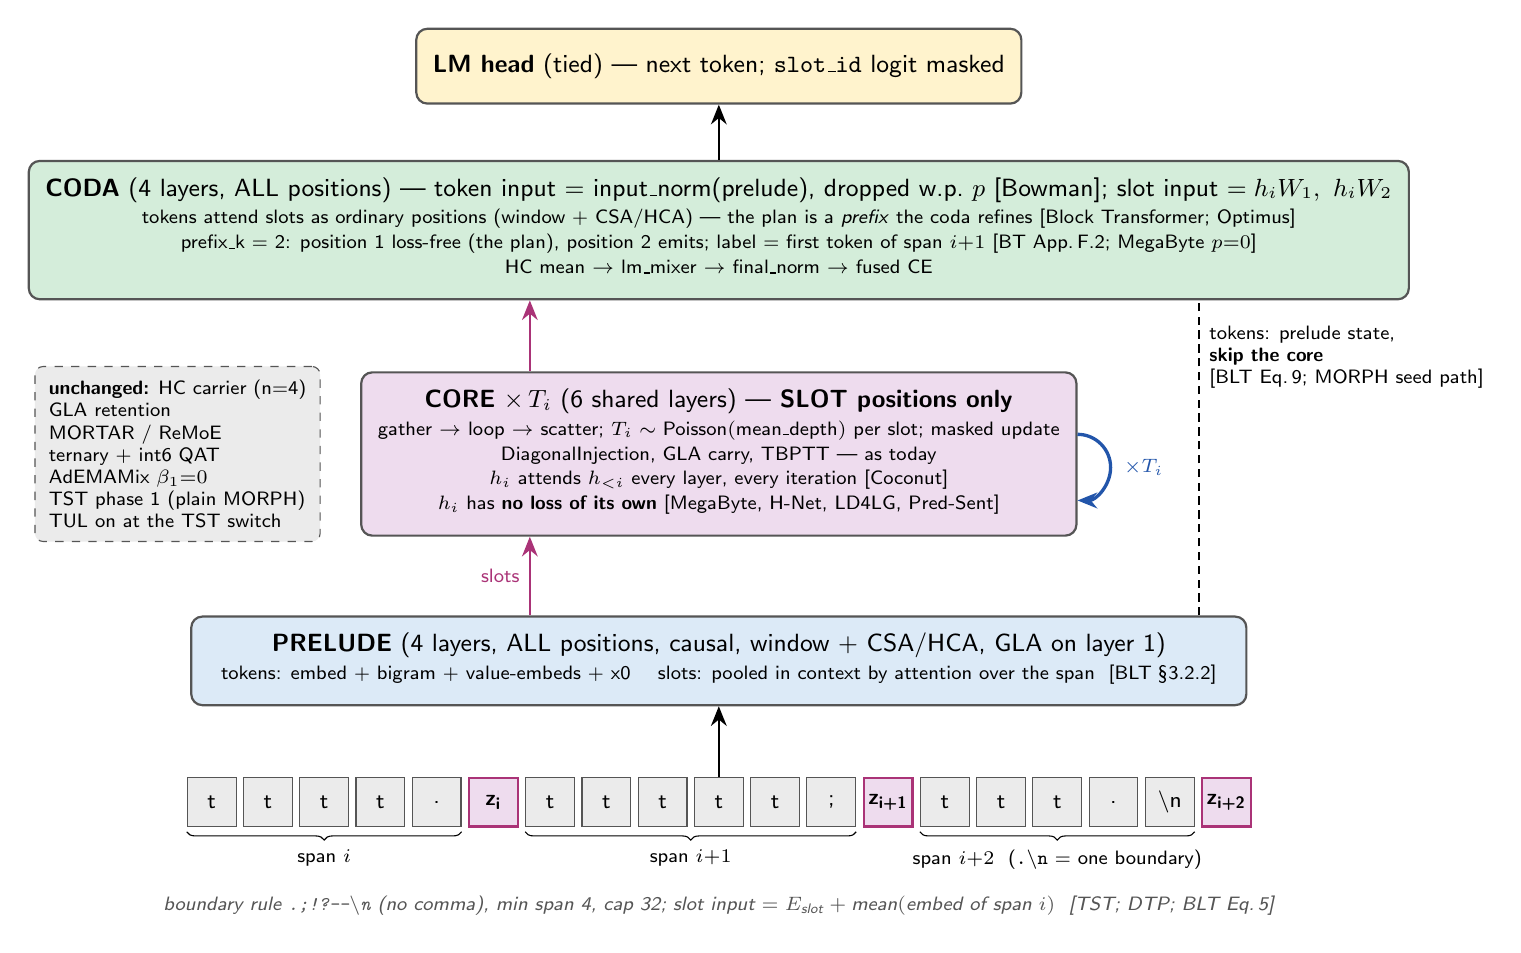
\begin{tikzpicture}[node distance=0.55cm and 0.4cm]

% ── input row: tokens with slots interleaved ────────────────────────────────
\node[tok] (t1) {t};
\node[tok, right=0.08cm of t1] (t2) {t};
\node[tok, right=0.08cm of t2] (t3) {t};
\node[tok, right=0.08cm of t3] (t4) {t};
\node[tok, right=0.08cm of t4] (t5) {.};
\node[slot, right=0.08cm of t5] (z1) {z\textsubscript{i}};
\node[tok, right=0.08cm of z1] (t6) {t};
\node[tok, right=0.08cm of t6] (t7) {t};
\node[tok, right=0.08cm of t7] (t8) {t};
\node[tok, right=0.08cm of t8] (t9) {t};
\node[tok, right=0.08cm of t9] (t10) {t};
\node[tok, right=0.08cm of t10] (t11) {;};
\node[slot, right=0.08cm of t11] (z2) {z\textsubscript{i+1}};
\node[tok, right=0.08cm of z2] (t12) {t};
\node[tok, right=0.08cm of t12] (t13) {t};
\node[tok, right=0.08cm of t13] (t14) {t};
\node[tok, right=0.08cm of t14] (t15) {.};
\node[tok, right=0.08cm of t15] (t16) {$\backslash$n};
\node[slot, right=0.08cm of t16] (z3) {z\textsubscript{i+2}};

\draw[decorate, decoration={brace, mirror, amplitude=3pt}] ($(t1.south west)+(0,-0.06)$) -- ($(t5.south east)+(0,-0.06)$)
  node[midway, below=3pt, sub] {span $i$};
\draw[decorate, decoration={brace, mirror, amplitude=3pt}] ($(t6.south west)+(0,-0.06)$) -- ($(t11.south east)+(0,-0.06)$)
  node[midway, below=3pt, sub] {span $i{+}1$};
\draw[decorate, decoration={brace, mirror, amplitude=3pt}] ($(t12.south west)+(0,-0.06)$) -- ($(t16.south east)+(0,-0.06)$)
  node[midway, below=3pt, sub] {span $i{+}2$ \ (\texttt{.}$\backslash$\texttt{n} = one boundary)};

\node[src, below=0.75cm of t9] (rule) {boundary rule \texttt{.;!?--\textbackslash n} (no comma), min span 4, cap 32; slot input $= E_{\text{slot}} + \text{mean}(\text{embed of span } i)$ \ [TST; DTP; BLT Eq.\,5]};

% ── PRELUDE ─────────────────────────────────────────────────────────────────
\node[B, fill=fBlue, minimum width=13.4cm, above=0.9cm of t9] (pre)
  {\textbf{PRELUDE} (4 layers, ALL positions, causal, window + CSA/HCA, GLA on layer 1) \\[-1pt]
   \begin{tabular}{@{}c@{}}\subf tokens: embed + bigram + value-embeds + x0 \quad slots: pooled in context by attention over the span \ [BLT §3.2.2]\end{tabular}};
\draw[A] (t9.north) -- (pre.south);

% ── CORE on slots only ──────────────────────────────────────────────────────
\node[B, fill=fPurple, minimum width=8.6cm, above=1.0cm of pre] (core)
  {\textbf{CORE} $\times\,T_i$ (6 shared layers) — \textbf{SLOT positions only} \\[-1pt]
   \begin{tabular}{@{}c@{}}\subf gather $\to$ loop $\to$ scatter; $T_i \sim \text{Poisson}(\text{mean\_depth})$ per slot; masked update\\[-2pt]
   \subf DiagonalInjection, GLA carry, TBPTT — as today\\[-2pt]
   \subf $h_i$ attends $h_{<i}$ every layer, every iteration [Coconut]\\[-2pt]
   \subf $h_i$ has \textbf{no loss of its own} [MegaByte, H-Net, LD4LG, Pred-Sent]\end{tabular}};
\draw[A, draw=cbPurple] ($(pre.north)+(-2.4,0)$) -- ($(core.south)+(-2.4,0)$) node[midway, left, sub, text=cbPurple] {slots};
\draw[A, draw=cbPurple] ($(core.north)+(-2.4,0)$) -- ($(core.north)+(-2.4,0.9)$);
% loop arrow on the core
\draw[A, draw=loopC, line width=1.2pt] ($(core.east)+(0,0.25)$) arc (90:-90:0.42) node[midway, right=1pt, sub, text=loopC] {$\times T_i$};

% tokens bypass the core
\draw[Ad] ($(pre.north)+(6.1,0)$) -- ($(pre.north)+(6.1,4.55)$) node[pos=0.72, right, sub, align=left] {tokens: prelude state,\\ \textbf{skip the core}\\ {[BLT Eq.\,9; MORPH seed path]}};

% ── CODA ────────────────────────────────────────────────────────────────────
\node[B, fill=fTeal, minimum width=13.4cm, above=0.9cm of core] (coda)
  {\textbf{CODA} (4 layers, ALL positions) — token input $=$ input\_norm(prelude), dropped w.p.\ $p$ [Bowman]; slot input $= h_i W_1,\ h_i W_2$ \\[-1pt]
   \begin{tabular}{@{}c@{}}\subf tokens attend slots as ordinary positions (window + CSA/HCA) — the plan is a \emph{prefix} the coda refines [Block Transformer; Optimus]\\[-2pt]
   \subf prefix\_k = 2: position 1 loss-free (the plan), position 2 emits; label = first token of span $i{+}1$ [BT App.\,F.2; MegaByte $p{=}0$]\\[-2pt]
   \subf HC mean $\to$ lm\_mixer $\to$ final\_norm $\to$ fused CE\end{tabular}};

% ── head ────────────────────────────────────────────────────────────────────
\node[B, fill=fYellow, minimum width=6.0cm, above=0.7cm of coda] (head)
  {\textbf{LM head} (tied) — next token; \texttt{slot\_id} logit masked};
\draw[A] (coda.north) -- (head.south);

% ── side note: what stays ───────────────────────────────────────────────────
\node[draw=bdr, dashed, rounded corners=3pt, fill=fGray, align=left, font=\scriptsize\sffamily,
      inner sep=5pt, left=0.5cm of core] (stay)
  {\textbf{unchanged:} HC carrier (n=4)\\ GLA retention \\ MORTAR / ReMoE \\ ternary + int6 QAT \\ AdEMAMix $\beta_1{=}0$ \\ TST phase 1 (plain MORPH) \\ TUL on at the TST switch};

\end{tikzpicture}
\end{document}
